main.tex\documentclass[a4paper]{article}
\usepackage[a4paper, margin=1.5in]{geometry}
\usepackage[utf8]{inputenc}
\usepackage{graphicx} % Required for inserting images
\usepackage[czech]{babel}
\usepackage{amsmath}
\usepackage{amssymb}
\usepackage[T1]{fontenc}
\usepackage{csquotes}
\usepackage{rotating}
\usepackage{hyperref}

\usepackage{lscape}
\usepackage{amsthm}
\usepackage{tikz}
\usetikzlibrary{automata,positioning}
\newtheorem*{statement}{Tvrzení}
\theoremstyle{definition}
\newtheorem*{solution}{Řešení}
\newcommand{\Mod}[1]{
\ \mathrm{mod}\ #1}
%\renewcommand\qedsymbol{\large{$\mathbb{Q.E.D.}$}}
\renewcommand\qedsymbol{\raisebox{-3mm}{\includegraphics[height=6mm]{koteseni.png}}}
\usepackage[parfill]{parskip}
\title{SFC projekt: Demonstrace činnosti GRU sítě}
\author{Bc.\ Vojtěch Vlach (\texttt{xvlach22})}
\newcommand{\rel}[1]{&(x \in #1 \wedge y \in #1)}
\date{2023/24}

\begin{document}

\maketitle

\section{Úvod}
V tomto projektu jsem se rozhodl demonostrovat činnost GRU sítě pomocí jazykové úlohy. A to rozdělování slov na slabiky, vytvořil jsem si vlastní dataset a využil jsem implementaci GRU v  knihovně PyTorch, pro trénování jsou využil domácí počítač bez GPU a částečně Google Colab s GPU runtime.

\section{Popis úlohy}

Pro tento projekt jsem si zvolil úlohu rozdělení slova na slabiky. Omezil jsem se pouze na české slova, kde mohu aspoň trochu posoudit správnost intuitivně. Přesněji se tedy jedná o problém, kde na vstupu je české slovo a na výstupu by mělo být slovo rozdělené na slabíky. Nenalezl jsem mnoho literatury, která by se tímto problémem zabývala, předpokládám, že je to úloha moc jednoduchá na to, aby se na tom dal zveřejňovat seriózní článek. Výjimku tvoří např. Hyphenation using Deep Neural Network\footnote{\href{https://negedng.github.io/files/2018-Hyphenation.pdf}{Gergely et al. Hyphenation using Deep Neural Network}}.

\subsection{Získání datasetu}

Pro výrobu datasetu jsem využil fonetický korpus Češtiny\footnote{\href{https://ujc.avcr.cz/phword}{The Phonological Corpus of Czech}}, který se zabývá kromě fonetické výslovnosti češtiny také četnostmi výskytu fonémů, slov a slabik. Konkrétně jsem využil následující sadu: \href{http://www.ujc.cas.cz/phword/ssc_29-06-16.zip}{Lexemes from Slovník spisovné češtiny, 4th edition, 2005}, která obsahuje právě fonetický přepis a jeho rozdělení na slabiky, které jsem využil. Slova v datasetu byly ve formátu, které jsou naznačeny ve sloupcích \texttt{Původní slovo}, \texttt{Fonetický přepis} a \texttt{Fonetické slabiky} viz tabulka \ref{table:dataset}.

Z těchto sloupců jsem jednoduchým algoritmem získal přepis na slabiky. Program procházel sloupce \texttt{Původní slovo} a \texttt{Fonetické slabiky} současně, nahrazoval fonetické výrazy původními písmeny a zanechal u nich informaci o slabikách. Více viz Python Notebook \texttt{python-scripts/Dataset\_creating.ipynb}.

Pro vytvoření samotných vstupů sítě a ground-truths jsem zvolil postup, kde síť detekuje konec slabiky a poslední písmeno nahradí příslušným tokenem (\texttt{@}). Doplnění oddělovače do výsledného slova (např. \texttt{-}) zajistí jednoduchý algoritmus. Tento způsob jsem zvolil proto, aby se nezpožďovaly výstupní písmena od těch vstupních. Tímto způsobem se síť může učit závislost pouze na několika málo posledních znacích. V opačném případě by zde vznikala závislost na znacích s větším rozestupem, což teoreticky zesložiťuje úlohu. Výsledkem tohoto zpracování byly sloupce \texttt{Vstup při trénování} a \texttt{Ground truth}, viz tabulka \ref{table:dataset}

\begin{table}[]
\centering
\caption{Tabulka 1: Proces získání datové sady.}
\begin{tabular}{|l|l|l|}
\hline
\textbf{Původní slovo}     & \textbf{Fonetický přepis}    & \textbf{Fonetické slabiky} \\ \hline
adresa                     & adresa                       & a.dre.sa                   \\ \hline
antimilitaristický         & antimilitariStiTSkí          & an.ti.mi.li.ta.riS.tiTS.kí \\ \hline
antikvariát                & antikvarijáT                 & an.ti.kva.ri.jáT           \\ \hline
popřípadě                  & popřípaďe                    & po.pří.pa.ďe               \\ \hline
\textbf{Přepis na slabiky} & \textbf{Vstup při trénování} & \textbf{Ground truth}      \\ \hline
a-dre-sa                   & adresa                       & @dr@sa                     \\ \hline
an-ti-mi-li-ta-ris-tic-ký  & antimilitaristicky           & a@t@m@l@t@ri@ti@ky         \\ \hline
an-ti-kva-ri-át            & antikvariat                  & a@t@kv@r@@t                \\ \hline
po-pří-pa-dě               & popripade                    & p@pr@p@de                  \\ \hline
\end{tabular}
\label{table:dataset}
\end{table}

\section{Implementace}
Všechny implementované skripty popsané v této kapitole jsou k nalezení ve složce \texttt{src}.

Pro svoji implementaci jsem se inspiroval článkem Gated Recurrent Unit (GRU) With PyTorch\footnote{\href{https://blog.floydhub.com/gru-with-pytorch/}{Loye Gabriel, 2019: Gated Recurrent Unit (GRU) With PyTorch}}, který ukazuje možnost využití pro predikci časové řady. Jeho řešení jsem si upravil, aby vyhovovalo mojí úloze.

\paragraph{GRUNet.}
Základní část mé implementace je třída \texttt{GRUNet} (viz soubor \texttt{src/gnu\_pytorch.py}, která definuje jednoduchou rekurentní síť s plně propojenou vrstvou na výstupu. Struktura sítě je definována jako GRU vrstva (+ ReLU aktivace) a plně propojená vrstva pro agregování vektoru skrytého stavu na formát výstupu. Vizualizování na Obrázku \ref{png:gru_adresa}.

\begin{figure*}[t!]
  \centering
  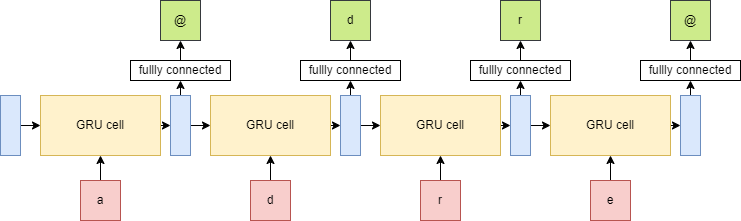
\includegraphics[width=4.5in]{gru_diagram_adresa.png}\\[1pt]  % width=\linewidth,hineight=1.7in
  \caption{Obrázek 1: Znázornění začátku činnosti sítě pro slovo \texttt{adresa}.\\Červená: vstup, žlutá: GRU buňka, bílá: plně propojená vrstva, modrá: vektor skrytého stavu, zelená: výstup sítě.}
  \label{png:gru_adresa}
\end{figure*}

\paragraph{Funkce train.}
Dále jsem naimplementoval funkci train, která spouští trénování pomocí zadaných paramterů. Umožňuje procházet dataset rozdělený na dávky a pro každý spočítá chybu a provede optimalizační krok. Jako chybovou funkci využívá \texttt{Mean\ Square\ Error} a k optimalizačním krokům využívá optimalizátor \texttt{Adam}, Dále umožňuje nahrát dříve uložený model a pokračovat v trénování. V průběhu shromažďuje statistiky o chybách a jednou za \texttt{save\_step} epoch uloží aktuální stav modelu a grafy znázorňující průběh chyby na trénovací i validační sadě.

\paragraph{Další drobnosti.}
Další části důležité pro běh trénování jsou tyto soubory \texttt{charset.py} (obsahující definici kódování slov ze \texttt{stringu} na \texttt{float tensor}), \texttt{helpers.py} (obsahující podpůrné funkce pro trénování: počítání levenshteinovy vzdálenosti, ukládání a nahrávání modelu a vytváření grafů), \texttt{dataset.py} (obsahující stejnojmennou třídu, která nahrává soubor a zpracovává ho na vstupy sítě a ground-truths a poskytuje možnost iterování přes batche),


\section{Spuštění + ovládání}

Pro spuštění by měl stačit python3.8+. První krok je nainstalování všech potřebných knihoven pomocí skriptu \texttt{install.sh}. Dále stačí spouštět skripty pomocí příkazové řádky.

Pro spuštění trénování je následující příkaz: \\
\texttt{python3 src/gru\_pytorch.py}

Tento příkaz spustí trénování podle nastavených parametrů přímo v kódu, např: \\
\texttt{train(trn\_dataset, val\_dataset, learn\_rate=0.001, device=device, \\
batch\_size=64, epochs=4000, save\_step=500, view\_step=100, \\
load\_model\_path='models')}

Pro manuální testování modelu je připraven soubor \texttt{src/inference.py}, který nabízí jednoduchý CLI interface k modelu. Je spustitelný pomocí příkazu: \\
\texttt{python3 src/ingerence.py}

pozn. pro úpravy a spouštění python notebooku \texttt{Dataset\_creating.py} je navíc potřeba prostředí pro Jupyter Notebook.

\section{Zhodnocení}
V požadovaném čase se mi nepodařilo natrénovat model, který by měl uspokojivé výsledky, ale podle grafu níže graf na Obrázku \ref{png:graf_trenovani} lze vidět, že pomocí trénování se model postupně zlepšoval a kdyby měl více času, nebo lepší hardware, je možné, že by dosáhl i lepších výsledků.

V tomto stavu se tedy lze bavit pouze o demonstraci postupného zmenšování chyby, ale nikoliv praktického použití. Příklady viz Tabulka \ref{table:vystupy}


\begin{figure*}[t!]
  \centering
  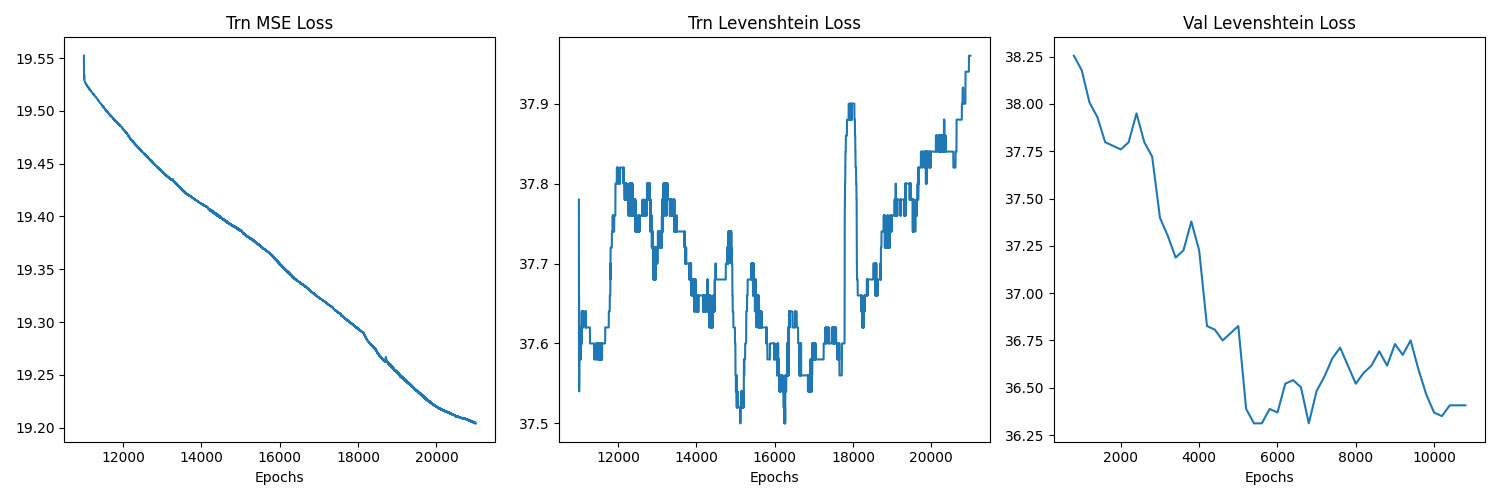
\includegraphics[width=4.5in]{torch_gru_8hid_250batch_21000epochs_losses.png}\\[1pt]  % width=\linewidth,hineight=1.7in
  \caption{Obrázek 2: Průběh trénování. Zleva: Průběh chyby Mean-Square-Error, průběh Levenshteinovy vzdálenosti na trénovací sadě, průběh Levenshteinovy vzdálenosti na validační sadě.}
  \label{png:graf_trenovani}
\end{figure*}


\begin{table}[]
\caption{Tabulka 2: Příklad výstupů nedotrénovaného modelu.}
\begin{tabular}{|l|l|l|}
\hline
\textbf{Vstup} & \textbf{Ground-truth}               & \textbf{Výstup}                     \\ \hline
vyhotovovat    & v@h@t@v@vat\_\_\_\_\_\_\_\_\_       & uxquvvuuvdt\_\_\_\_\_\_\_\_\_       \\ \hline
cecko          & ce@ko\_\_\_\_\_\_\_\_\_\_\_\_\_\_\_ & epmnu\_\_\_\_\_\_\_\_\_\_\_\_\_\_\_ \\ \hline
vynalez        & v@n@lez\_\_\_\_\_\_\_\_\_\_\_\_\_   & uxrtnpw\_\_\_\_\_\_\_\_\_\_\_\_\_   \\ \hline
\end{tabular}
\label{table:vystupy}
\end{table}

\end{document}
